\documentclass[10pt]{article}

\usepackage{algorithm,algpseudocode}
\usepackage{a4wide,amsmath,amssymb,fancyhdr,graphicx,tabularx,xspace}
\usepackage{tikz}
\usetikzlibrary{arrows.meta}
%------------------------------------------------------------------------------
\newcommand{\course}{}
\newcommand{\coursenumber}{}
\newcommand{\courseyear}{}
%------------------------------------------------------------------------------
\pagestyle{fancy}
\chead{}
\lhead{-}
\rhead{\course\ Text Assignment \courseyear}
\cfoot{\thepage}
\lfoot{}
\rfoot{}
%------------------------------------------------------------------------------

%to include IPE/pdf correctly
\expandafter\ifx\csname pdfoptionalwaysusepdfpagebox\endcsname\relax\else
\pdfoptionalwaysusepdfpagebox5
\fi


\newcommand{\Reals}{{\Bbb R}}
\newcommand{\Nats}{{\Bbb N}}
\newcommand{\Ints}{{\Bbb Z}}

\newcommand{\C}{\ensuremath{\mathcal{C}}}
\newcommand{\E}{\ensuremath{\mathcal{E}}}
\newcommand{\F}{\ensuremath{\mathcal{F}}}
\newcommand{\G}{\ensuremath{\mathcal{G}}}
\newcommand{\U}{\ensuremath{\mathcal{U}}}

\newcommand{\graph}{\ensuremath{\mathcal{G}}}
\newcommand{\tree}{\ensuremath{\mathcal{T}}}
\newcommand{\node}{\nu}
\newcommand{\lchild}{\mathrm{lc}}
\newcommand{\rchild}{\mathrm{rc}}
\newcommand{\size}{\mathit{size}}
\newcommand{\leaf}{\mu}
\newcommand{\mylist}{{\cal L}}
\newcommand{\myroot}{\mathit{root}}
\newcommand{\key}{\mathit{key}}
\newcommand{\bd}{\partial}

\newcommand{\myopt}{\mbox{{\sc opt}}\xspace}
\newcommand{\lb}{\mbox{{\sc lb}}\xspace}
\newcommand{\loadb}{{\sc Load Balancing}\xspace}

\newcommand{\vc}{{\sc Vertex Cover}\xspace}
\newcommand{\wvc}{{\sc Weighted Vertex Cover}\xspace}
\newcommand{\wsetc}{{\sc Weighted Set Cover}\xspace}
\newcommand{\tsp}{{\sc TSP}\xspace}
\newcommand{\mst}{{\sc MST}\xspace}

\newcommand{\eps}{\varepsilon}
\newcommand{\ol}{\overline}
\renewcommand{\leq}{\leqslant}
\renewcommand{\geq}{\geqslant}

\newcommand{\pr}[1]{\Pr[#1]}
\DeclareMathOperator{\expectation}{E}
\newcommand{\expt}[1]{\expectation[#1]}
\newcommand{\events}[1]{\mbox{Events}(#1)}
\newcommand{\rank}{\mathit{rank}}
\newcommand{\result}{\mathit{result}}
\newcommand{\piv}{\mathrm{piv}}
\newcommand{\myexp}{\mathrm{exp}}
\newcommand{\best}{\mathrm{best}}
\newcommand{\worst}{\mathrm{worst}}
\newcommand{\dest}{\mathit{dest}}
\newcommand{\dist}{\mathit{distance}}
\newcommand{\weight}{\mathit{weight}}
\newcommand{\mylength}{\mathit{length}}
\newcommand{\length}{\mathit{length}}
\newcommand{\alg}{{\sc Alg}\xspace}

\newcommand{\start}{\mathit{start}}
\newcommand{\myend}{\mathit{end}}
\newcommand{\free}{\mathit{free}}
\newcommand{\true}{{\sc True}\xspace}
\newcommand{\false}{{\sc False}\xspace}

\newcommand{\etal}{{\emph{et al.}\xspace}}


%------------------------------------------------------------------------------
% Theorem-Like Environments
%------------------------------------------------------------------------------
\newtheorem{defin}{Definition}
\newenvironment{mydefinition}{\begin{defin} \sl}{\end{defin}}
\newtheorem{theo}[defin]{Theorem}
\newenvironment{mytheorem}{\begin{theo} \sl}{\end{theo}}
\newtheorem{lem}[defin]{Lemma}
\newenvironment{mylemma}{\begin{lem} \sl}{\end{lem}}
\newtheorem{propo}[defin]{Proposition}
\newenvironment{myproposition}{\begin{propo} \sl}{\end{propo}}
\newtheorem{coro}[defin]{Corollary}
\newenvironment{corollary}{\begin{coro} \sl}{\end{coro}}

\newenvironment{myproof}{\emph{Proof.}}{\hfill $\Box$ \medskip\\}

%------------------------------------------------------------------------------
\newcounter{rcounter}
\newenvironment{rlist}%
{\begin{list}{\setnr-\arabic{rcounter}}{\usecounter{rcounter}}}{\end{list}}
\newcounter{rcountermem}
%------------------------------------------------------------------------------

\title{Solutions}
\author{Natasja van de L'Isle - 1022588}
\date{18/02/2016}


\begin{document}
	
	
	%------------------------------------------------------------------------------
	\newcommand{\setnr}{Exercise}
	\subsection*{Exercises}
	%------------------------------------------------------------------------------
	\begin{rlist}
\item

\begin{figure}[ht]
\centering
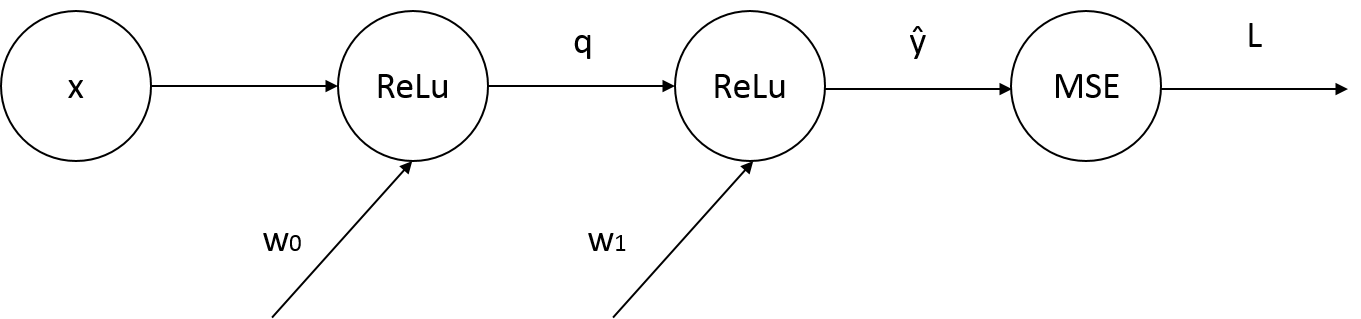
\includegraphics[width=0.75\textwidth]{Q1_graph}
\caption{Graph}
\end{figure}

We can use two approaches to compute new values for the weights $w_0$ and $w_1$. The first one is to update the weights after each observation. The second is to take the average of the computed weights and thus, only update once.

Observations: $(x_1,y_1) = (1,2)$ and $(x_2,y_2) = (2,3)$
Weights: $w_0 = 1$ and $w_1 = 2$

We use the MSE as loss function: $L = \frac{1}{2} (\hat{y}-y)^2$

%$L = \frac{1}{2n}\sum_{i=0}^n(\hat{y}_i-y_i)^2$

The first approach: 
\begin{flalign}
\hat{y}_1 &= w_1(w_0x_1)\\
	&= 2*1*1 = 2\\
L &= \frac{1}{2}(2-2)^2\\
	& = 0\\
\end{flalign}

As $L=0$ the derivatives will all be zero and, therefore, the weights will not be updated. Thus, we continue to the next observation.

\begin{align*}
\hat{y}_2 &= w_1(w_0x_2)\\
	&= 2*1*2 = 4\\
L &= \frac{1}{2}(4-3)^2 = \frac{1}{2}\\
\frac{\partial L}{\partial \hat{y_2}} &= [\frac{1}{2} (\hat{y_2}-y_2)^2]'\\
	&= 2*\frac{1}{2} (\hat{y_2}-y_2) * 1\\
	&= \hat{y_2}-y_2 \\
	&= 1\\
\frac{\partial L}{\partial w_1} &= \frac{\partial \hat{y_2}}{\partial w_1} \frac{\partial L}{\partial \hat{y_2}}\\
	&=  w_0x_2*\frac{\partial L}{\partial \hat{y_2}}\\
	&=  2*\frac{1}{2}\\
	&= 1\\
\frac{\partial L}{\partial q} &= \frac{\partial \hat{y_2}}{\partial q} \frac{\partial L}{\partial \hat{y_2}}\\
	&= w_1 * 1\\
	&= 2\\
\frac{\partial L}{\partial w_0} &= \frac{\partial q}{\partial w_0} \frac{\partial L}{\partial q}\\
	&= x_2 *\frac{\partial L}{\partial q}\\
	&= 2*2 = 4
\end{align*}

Thus, $w_1^* = w_1-0.1*2 = 1.8$ and $w_0^* = w_0 - 0.1*4 = 0.6$.



\item
Various decisions need to be made in a modeling process to address specific properties of the data and the modeling goal. In this task, you are given a description of a data structure and a goal for which you need to design a model. 

Produce a figure depicting your model. Briefly explain the figure and justify all decisions made in the modeling process. In detail, describe at least: 
- Input data format
- Number of layers
- Type of layers (Dense, Recurrent, Convolutional - 1D, 2D, 3D)
- Regularization
- Model output ----- caption? 
- Loss function  ---- 0/1 loss


The training and execution procedures for the model may differ, so you can use different descriptions for both. 

*Data and goal description:*

The goal of this task is to generate captions for short video clips. 

The video data is structured as sequences of color images. The model needs to be able to process a number of consecutive images that form a short video clip. The training data consists of video clips (few seconds) and a short caption (5-10 words). 

For simplicity, the accuracy of the model is evaluated on the exact prediction of the caption. In other words, the model needs to produce correctly the specific words in a specific order for each video. 


\begin{itemize}
\item Input data format: The data format will be a tensor of images. Each image is 3D, thus each sequence of images for each video will be 4D tensor. 

\item Number of layers: The model consists of two layers. A CNN and a RNN layer.

\item Type of layers: 
\begin{enumerate}
\item CNN layer. The setup of the CNN is as we have seen in the lecture, type D. However, we end with with a singel vector after the two FC 4096. Hence, we do not have the FC 1000 and softmax at the end. Thus, for each image we run a CNN, each image becomes a FC 4096. Then we run a mean pooling over it to get one vector representing the total video. We choose to to a mean pooling afterwards, because we want the mean image of the video. For example, the video shows a boy playing football. However, the video shows the ball and the boy most of the time but there is also a lot of noise on the background clearly visible in some images. We then want to take the average such that every part of the video is captured by the FC 4096. Thus, the vector is a summary of the entire video. This single vector is then the input for the next layer.

This can be seen in figure BLABLABLA

\item RNN layer. This layer consists of the a recurrent neural network using the LSTM setup for each cell. The main idea here is to generate a word at each time stamp. This word comes from a dictionary on which the model is already pre-trained. The input at each cell is the output from the previous cell and the summary vector of the images. The output is a word that is choses with the highest probability: $\max \Pr[\text{word}_i|\text{previous words chosen}]$.

This can be seen in figure BLABLABALA
\end{enumerate}

\item Regularization:  ?????????????????????

\item Model output: The model outputs a sequence of words. This sequence is smaller than or equal to 10. 

\item Loss function:
The loss function is the 0/1-loss function as we want the exact caption. Thus, if the caption that is ouputted is only slighly off, the loss will still equal one as it is not completely correct. 

\end{itemize}



	\end{rlist}

\end{document}